\chapter{Cibles de fonctionnement}

\section{Les attentes client}

Nous avons été contactés par la société SPIE Sud-Est afin d'améliorer certains points dans le processus de gestion des contrats de maintenance. Il s'agit de proposer des solutions pour : 

\begin{itemize}
    \item développement de procédures métier et de supports d'exploitation par les entités de maintenance et service
    \item standardisation des procédures métier et de supports d'exploitation pour les entités exerçant le même métier sur le même secteur d'activité client
    \item analyse des risques propres à chaque métier sur le même secteur d'activité client
    \item amélioration de la définition des limites des interfaces avec les autres processus
    \item mise en place d'un Info centre dur l'intranet
\end{itemize}

Les chapitres précédents --- analyse de l'existant et benchmarking -- permettent d'identifier quelques axes sur lesquels le système d'information de SPIE péche contre les bonnes pratiques et où des améliorations sont à prévoir.

    Nous allons donc citer dans ce document certains thèmes d'amélioration possibles à travers les axes suivant:

    \begin{enumerate}
        \item Identification de nouvelles technologies à forte valeur ajoutée~;
        \item Réorganisation des acteurs des processus métiers de SPIE pour suivre les ``best-practices'' dégagées~;
        \item Réorganisation de la logique des processus existants~;
    \end{enumerate}

\section{Réorganisation des processus}

\subsection{Processus Retour d'expérience}

\begin{figure}[h!]
	\centering
	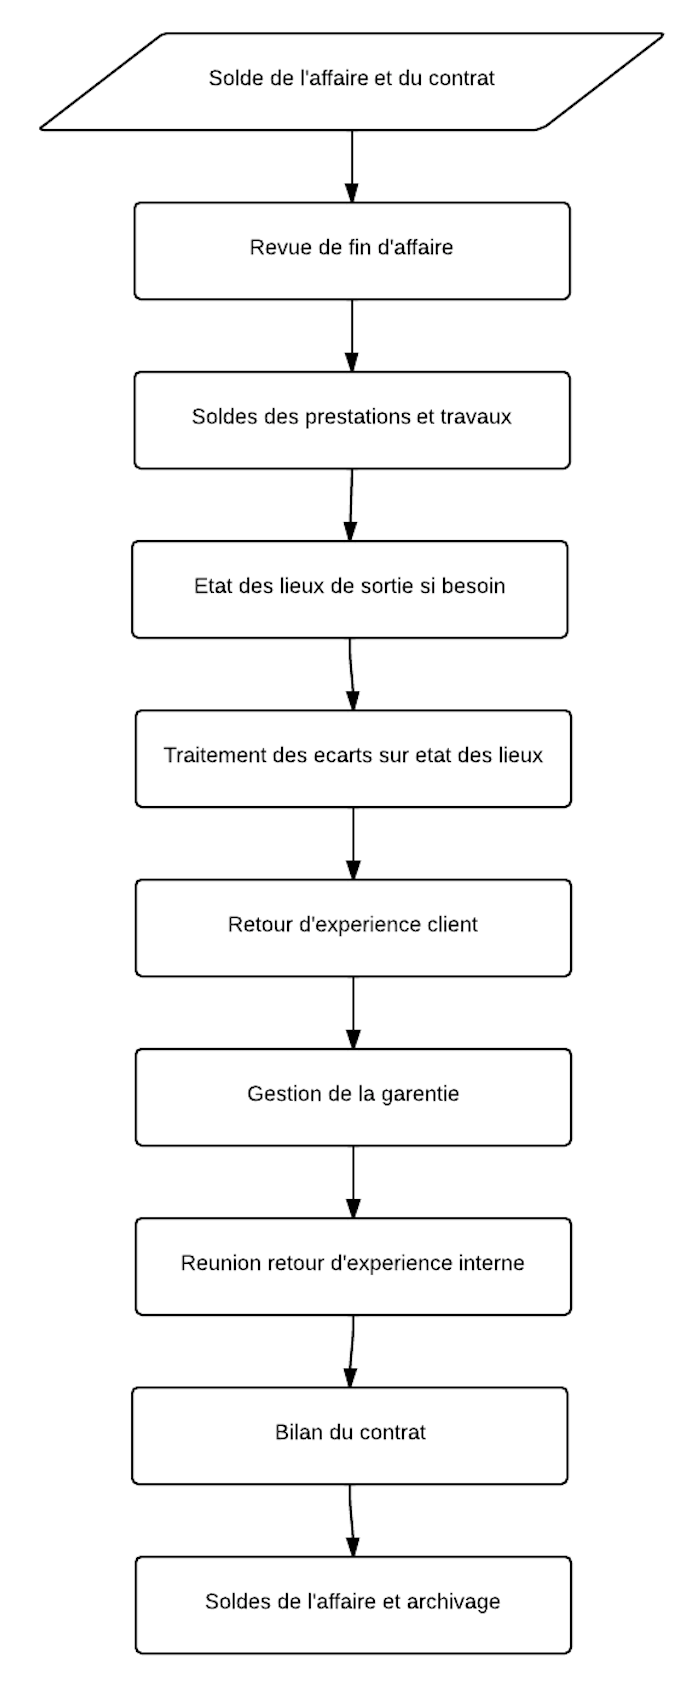
\includegraphics[width=0.45\linewidth]{images/processus_retour_experience.png}
	\caption{Processus de retour d’expérience}
	\label{fig:processusRetourExperience}
\end{figure}

Ainsi l'ajout du processus \textit{retour d'\'exp\'erience client} dans le sous-processus \textit{solde
de l'affaire et du contrat} r\'epond aux exigences de SPIE Sud Est suivante~:

\begin{itemize}
    \item Base de connaissance m\'etier type de contrat~;
    \item Identification des risques techniques/financiers/organisationnels.
\end{itemize}


\subsection{Revue des processus}

A fins d'armoniser les retours d'experience, et s'assurer que chaque remarques d\'eduites des autres processus
soient appliqu\'e au ceux en cours, nous decidons de cr\'eer un tout nouveau processus completement parrallele
\`a ceux d\'ej\`a existant.

\begin{figure}[h!]
	\centering
	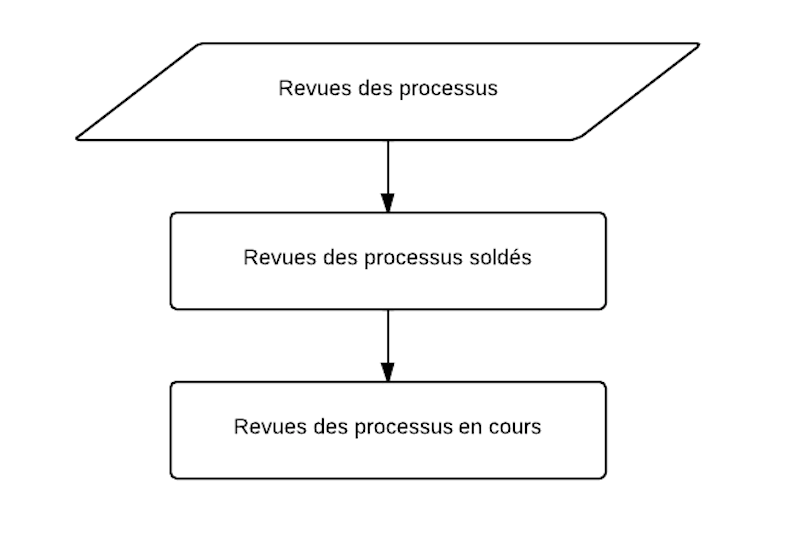
\includegraphics[width=0.45\linewidth]{images/processus_revues.png}
	\caption{Processus de revues}
	\label{fig:processusRevue}
\end{figure}

